\documentclass[sigconf,nonacm]{acmart}

\usepackage[textsize=small]{todonotes}
\usepackage{subcaption}
\usetikzlibrary{3d, arrows.meta, positioning}
\usepackage{tabularray}
\UseTblrLibrary{amsmath,booktabs,counter,diagbox,nameref,siunitx,varwidth,zref}
\pgfkeys{tikz/.cd,
box color/.code={\xdef\tkzThreedBoxColor{#1}},
box color=white
}
\def\parsexy(#1,#2,#3){(#1,#2)}
\def\parsexz(#1,#2,#3){(#1,#3)}
\def\parseyz(#1,#2,#3){(#2,#3)}
\def\parsex(#1,#2,#3){#1}
\def\parsey(#1,#2,#3){#2}
\def\parsez(#1,#2,#3){#3}

\newcommand{\tkzThreeDBox}[5][white]{\tikzset{#1}
\edef\temp{%
\noexpand\filldraw[#1,fill=\tkzThreedBoxColor!40,canvas is yz plane at x=\parsex#3+\parsex#2] 
\parseyz#2 rectangle (\parsey#4+\parsey#2,\parsez#5+\parsez#2);
\noexpand\filldraw[#1,fill=\tkzThreedBoxColor!30,canvas is xz plane at y=\parsey#4+\parsey#2] 
\parsexz#2 rectangle (\parsex#3+\parsex#2,\parsez#5+\parsez#2);
\noexpand\filldraw[#1,fill=\tkzThreedBoxColor!50,canvas is xy plane at z=\parsez#5+\parsez#2] 
\parsexy#2 rectangle (\parsex#3+\parsex#2,\parsey#4+\parsey#2);
}
\temp
}


\usepackage{caption}

\def\div{\mathrm{div}}
\def\O{\mathcal{O}}
\newcommand{\norm}[1]{\left\lVert#1\right\rVert}

\bibliographystyle{alpha}
\title[Geodesic Paths and Distances on Meshes]{Geodesic Paths and Distances on Meshes\texorpdfstring{: PDE and
Computational Geometry Approaches\\{\normalsize Report on \textit{A Survey of 
Algorithms for Geodesic Paths and Distances}}}{}}


\author{Matthieu Pierre Boyer}
\authornote{Both authors contributed equally.}
\affiliation{%
	\institution{École Normale Supérieure}
	\city{Paris}
	\country{France}}
\email{matthieu.boyer@ens.fr}

\author{Antoine Groudiev}
\authornotemark[1]
\affiliation{%
	\institution{École Normale Supérieure}
	\city{Paris}
	\country{France}}
\email{antoine.groudiev@ens.fr}

\def\abs#1{\left|#1\right|}
\def\R{\mathbb{R}}

\def\V{\mathbb{V}}
\def\nv{n_{\V}}
\def\E{E}
\def\ne{n_{\E}}
\def\F{\mathcal{F}}
\def\nf{n_{\F}}
\def\d{\mathrm{d}}

\begin{abstract}
	In this report, we investigate different methods to compute shortest-paths
	on meshed $2$-manifolds embedded in $\R^{3}$, based on \cite{craneSurvey}.
	We will most notably compare different types of methods, either coming from
	the resolution of PDEs on the manifold, or through the unfolding of the embedding to $\R^{2}$.
	We also provide from-scratch implementations of five classes of methods, namely the heat method,
  the fast marching algorithm, the spectral embedding resistance distance transform,
  the Poisson equation border transform, and the Improved Chen-Han algorithm, and compare their 
  performances on several datasets.
	% for a blazingly fast™ result.
\end{abstract}

\begin{teaserfigure}
	\centering
	\includegraphics[height=5cm]{images/rabbit-paths.png}
	\hspace{1cm}
	\includegraphics[height=5cm]{images/venus-paths.png}
	\hspace{1cm}
	\includegraphics[height=5cm]{images/star-paths.png}
	\caption{Geodesic paths on meshes, computed with our implementation of the Improved Chen-Han algorithm. Faces are colored from red to green according to the distance of their barycenter to the source point. The geodesic path to each vertex is drawn in blue.}
	\Description{}
	\label{fig:teaser}
\end{teaserfigure}

\begin{document}
\maketitle

\section*{Introduction}
Computing the distance between two points and retrieving a shortest path is, in general, a fundamental problem in computer science. While the problem is well understood in flat, Euclidean spaces, as well as on graphs, it becomes more challenging when considering curved surfaces. Indeed, the geodesic distance between two points on a surface is defined as the length of the shortest path that lies entirely on the surface. Computing such distances and paths is a non-trivial task, even when the surface is represented as a discrete mesh.

Such a problem arises in various fields, including computer graphics, robotics, medical imaging, and computer vision. In computer graphics, geodesic distances are used for texture mapping \cite{oliveira2010geotextures}; in robotics, they form the cornerstone of path planning algorithms on complex terrains \cite{garrido2013application}; in medical imaging, they assist in analyzing anatomical structures \cite{miller2006geodesic}; and in computer vision, they improve object recognition and shape analysis \cite{shamai2017geodesic}.

The ability to efficiently compute geodesic distances and paths is therefore crucial for many applications in which the size of the problem is large, and where real-time performance is required. In the polyhedral setting, where the surface is represented as a mesh of vertices, edges, and faces, the number of vertices is derived from the desired accuracy of the representation, and can thus be very large. Algorithms with a low theoretical and practical complexity are therefore essential to handle such large-scale problems.

After brief mathematical reminders in \autoref{sec:math-reminders}, we present four classes of methods
based on the resolution of Partial Differential Equations (PDEs) in \autoref{sec:pde-methods}.
Then, in \autoref{sec:comp-geom-methods}, we discuss computational geometry methods, focusing on the Improved Chen-Han algorithm.
Finally, we present experiments and results in \autoref{sec:experiments}, and conclude in the final section.

\section{Mathematical reminders}
\label{sec:math-reminders}
Formally, a $2$-manifold (without boundary) is a topological space in which all points have neighborhoods
homeomorphic to disks (without boundary) in $\R^{2}$.
Such a homeomorphism is called a chart.
Intuitively, this means that zooming enough on any point of the manifold will make it look like a flat surface.
In \autoref{fig:manifolds-examples}, we can see that some meshes are not manifolds, as some points are locally non-flat.

\begin{figure}[ht]
	\centering
	\includegraphics[width=.4\linewidth]{images/manifold.png}
	\includegraphics[width=.5\linewidth]{images/nonmanifold.png}
	\caption{Examples of a $2$-manifold (left) and non-manifold (right) mesh. (Images generated from our custom viewer.)}
	\Description{}
	\label{fig:manifolds-examples}
\end{figure}

When considering a $2$-manifold $M$, a (smooth) curve is a (smooth) application $\gamma: I \to M$ for an interval $I$.
Two curves $\gamma_{1}, \gamma_{2}$ on the same interval $(-\epsilon, \epsilon)$ based at
$q = \gamma_{1}(0) = \gamma_{2}(0)$ are equivalent if, in some chart, they have same first Taylor expansion
around $0$.
Its tangent vector $\dot{\gamma}(0)$ at $q = \gamma(0)$ is the equivalence class\footnote{This allows us to
	define the (covariant) derivative of a vector field on a manifold, as well its gradient and Laplacian,
	but the mathematics behind these definitions are behind the scope of this report.} of $\gamma$ in the
space of smooth curves in $M$.
The tangent space at $q \in M$ is the set $T_{q}M$ of all tangent vectors of smooth curves based at $q$.
It has the structure of a $2$-dimensional vector space.
A Riemannian tensor $g$ on $M$ is an application which to $q \in M$ associates a positive definite symmetric
endomorphism of $T_{q}M$.
A $2$-manifold equipped with a Riemannian tensor $g$ is called a Riemannian $2$-manifold.
We can define the length of a curve $\gamma: [a, b] \to M$ on such a manifold as
\begin{equation}
	L(\gamma) = \int_{a}^{b}\sqrt{g_{\gamma(t)}\left(\dot{\gamma}(t), \dot{\gamma}(t)\right)}\d t.
\end{equation}
The geodesic (curve) between $p$ and $q$ is the curve $\gamma$ verifying
\begin{equation*}
	\gamma = \arg\min_{\gamma: [0, 1] \to M, \gamma(0) = p, \gamma(1) = q} L(\gamma).
\end{equation*}
The length of the geodesic between $p$ and $q$ is the called the geodesic distance.
As presented above, computing the geodesic curves and the geodesic distances has multiple applications,
and this is the problem we will be tackling in this report.

\smallskip

In our context, we will be given a $2$-manifold already meshed%
\footnote{\cite{craneSurvey} gives a few methods to create such a meshing.
	In particular, our implementations of the methods are restricted without loss of generality to triangular
	faces; more general meshes can be considered through triangulation techniques.}%
, that is, a finite set $\V \subseteq \R^{3}$ of vertices
(of cardinal $\nv$) and a finite set $\F \subseteq \left\llbracket 1, \nf\right\rrbracket^{3}$
of faces, given by the indices of the associated vertices.
The edges $\E$ of the manifold are given by any subsets of size two of a face $f \in \F$.
Because continuous functions on the manifold cannot be fully represented in memory, and especially by a
finite number of points on the mesh, functions on the manifold will be approximated by functions
on $\V$, on $\E$ or on $\F$.
As such, we will take any function and interpolate it linearly on each face, giving us a piecewise-linear
function.

A path on a piecewise-linear manifold can then be understood as interpolating on pieces of the manifold, or
directly computing the curves on the mesh.
The quality of the approximation by the mesh of the $2$-manifold will never be taken into account in the
quality results.
Finding the best approximation of a curved surface by a mesh is a whole other problem that we will not address in this report.

We now present two classes of methods to compute such geodesic paths and distances on a mesh.

\section{PDE-based methods}
\label{sec:pde-methods}
In this section we will study methods inspired by Partial Differential Equations (PDE) that arise from models
of physical phenomena.
Indeed, many physical phenomena propagate along the surfaces over time, and dissipate over space, thus
allowing us to retrieve geodesics from solutions to the equations.

\subsection{General Theory}
Consider the parabolic heat equation
\begin{equation*}
	\frac{\d}{\d t}u_{t} = \Delta u_{t}.
\end{equation*}
Here, $u_{t}$ is the temperature profile at time $t$ and $\Delta$ is the Laplacian operator (or divergence of the gradient operator).
However, on a piecewise-linear (PL) manifold, because functions on vertices are interpolated linearly to
become functions on the manifold, the gradient is piecewise-constant and can be computed explicitly from the
values at each vertex.
Consider a face $f \in \F$ with vertices $p_{i}, p_{j}, p_{k} \in \R^{3}$.
Let $e_{1} = p_{j} - p_{i}$ and $e_{2} = p_{k} - p_{i}$.
The face normal is
\begin{equation*}
	\overrightarrow{n_{f}} = \frac{e_{1} \times e_{2}}{\abs{e_{1} \times e_{2}}},
\end{equation*}
where $\times$ is the cross product in $\R^{3}$
and thus the gradient, being perpendicular to level curves is
\begin{equation}
	\nabla u_{\mid_{f}} = \frac{1}{2A_{f}}\sum_{l \in f}u_{l}(\overrightarrow{n_{f}}\times e_{l}), \label{eq:facegrad}
\end{equation}
where $A_{f} = \frac{1}{2}\abs{e_{1} \times e_{2}}$ is the area of face $f$ and $e_{l}$ is the \textbf{opposite} to vertex $l$.
Note that we can represent the gradient as a matrix $G \in \R^{\nv \times 3\nf}$, although this
representation is really inefficient for practical computation.
The definition of the divergence then comes from the Gauss-Ostrogradski theorem by intregration by parts
\begin{equation}
	\left(\nabla \cdot X\right)_{i} = \frac{1}{A_{i}}\sum_{f \ni i}\sum_{e \in f}\frac{1}{2}\cot{\left(\alpha_{e}^{f}\right)}\langle X_{f}, e\rangle, \label{eq:divergence}
\end{equation}
where $A_{i}$ is the Voronoi area associated with vertex $i$ and $\alpha_{e}^{f}$ is the angle at the vertex
opposite to edge $e$ in $f$.

Finally, we can define the Laplace-Beltrami operator (the PL version of the continuous Laplacian) as $\Delta = (\nabla \cdot) \circ \nabla : \V \to \R$ or simply
\begin{equation}
	(\Delta u)_{i} = \frac{1}{2A_{i}}\sum_{e = (i, j)}\left(\cot \alpha_{i, j} + \cot \beta_{i, j}\right)\left(u_{i} - u_{j}\right),\label{eq:Laplacian}
\end{equation}
where $\alpha_{i, j}, \beta_{i, j}$ are the two angles opposite edge $(i, j)$.
One could then see the Laplace-Beltrami operator as a matrix $L \in \R^{\nv \times \nv}$.

\smallskip

After the spatial discretization of the laplace operator we just described, operating a time discretization in a single
backward Euler step for some fixed time $t$ will give us approximate solutions to the equation.
If we want to find the distance maps from some set $X \subseteq \V$, we simply solve the linear equation
associated to the continuous equation we need to solve.

\subsection{Physical Equations}
In our implementation, we compared multiple methods based on physical phenomena allowing to trace geodesics,
or at least geodesic-like curves.
Indeed, not all of those compute the true geodesic distance, but some sense of distance that can be drawn
and integrated to find shortest paths.

\smallskip

The following equations all rely on the Laplace-Beltrami operator (or Laplacian operator $\Delta$) which
models the sum of second-order derivatives along each axis of a function.
It is not difficult to understand how such an operator can mimic the propagation of a phenomenon in space.
Indeed, the Laplacian of $u$ at $x$ measures the average extent of the deviation from the value of $u$ near
$x$ to the value of $u$ at $x$.
As such, when we consider systems in which some quantity at a point is influenced by the value of the same
quantity at nearby points (possibly with a time deviation), the Laplacian naturally occurs.
Adding this to the symmetry at the core of the Laplacian's definition (in a local coordinate frame), when the laws of deviation are symmetric, which is often the case in physics, the Laplacian is bound to appear.
From a more mathematical point of view, the Laplacian is the first scalar linear differential operator
being covariant\footnote{Considering the linear category of differential operators between tensor fields,
	we can prove that the Laplacian is generated by the covariant derivative ; which in Riemannian
	geometry can be thought as the derivative along a vector adjusted to respect the Riemannian tensor
	metric of the	manifold.}, and is fundamental as such.

\paragraph{Heat Method}
This method is based on the heat equation
\begin{equation}
	\nabla u_{t} = \frac{\d}{\d t}u_{0},\label{eq:heat}
\end{equation}
which models the
evolution of temperature profiles $u_{t}$ in time in a given material, which here will be our surface,
from the initial profile $u_{0}$.
It can be derived from the first principle of thermodynamics on infinitesimal slices of material and
describes the fact that spatial variations of temperature spread quadratically with regard to time.
This means that spreading temperature from point A to point B will take of the order of magnitude of the
square of the distance between A and B.
\begin{figure}[H]
	\centering
	\begin{tikzpicture}[x={(1,0)},z={(-1/3,-1/4)},y={(0,1)},font=\sffamily, scale=.9]
	\tkzThreeDBox[box color=orange,draw=none]{(0,0,0)}{(1,0,0)}{(0,2,0)}{(0,0,4)}
	\fill[orange!80,canvas is yz plane at x=1] (0.5,0.5) coordinate(X) rectangle ++(1,3);
	\shade[opacity=0.7,left color=orange!80,right color=blue!50!cyan!60!white,canvas is xy plane at z=0.5]
	(1,0.5) rectangle ++(6,1);
	\shade[opacity=0.7,left color=orange!80,right color=blue!50!cyan!60!white,canvas is xz plane at y=0.5]
	(1,0.5) rectangle ++(6,3);
	\shadedraw[draw=red!50,left color=orange!15,right color=orange!40]
	(1.5,.15,1) --  (1.5,.85,1) -- plot[variable=\x,domain=0:3,samples=60]
	(\x+1.5,{.85+0.1*sin(720*\x/3)},1) --++(0,0.25,0) -- ++(0.5,-0.6,0)
	-- ++(-0.5,-0.6,0) --++(0,0.25,0)
	-- plot[variable=\x,domain=3:0,samples=60]
	(\x+1.5,{0.15+0.1*sin(720*\x/3)},1) -- cycle;
	\draw[dashed,draw=orange!20,thick] (X) -- ++(6,0,0);
	\tkzThreeDBox[box color=white,fill opacity=0,draw=orange!20,thick]{(1,0.5,0.5)}{(6,0,0)}{(0,1,0)}{(0,0,3)}
	\tkzThreeDBox[box color=cyan,draw=none]{(7,0,0)}{(1,0,0)}{(0,2,0)}{(0,0,4)}
	\node at (0.5,1,4) {$T_2$};
	\node (Q) at (3.5,.75,2) {$\delta Q = -\frac{\partial T}{\delta x}$};
	\node at (7.5,1,4) {$T_1$};
	\draw[{Bar}{Latex}-{Latex}{Bar}] (1,.3,4) -- (7,.3,4) node[midway,fill=white]{$\delta x$};
	\node[above=1cm of Q,draw] {$T_2>T_1$};
\end{tikzpicture}


	\caption{Illustration of the heat propagation between two slices of material of temperatures $T_2$ and $T_1$.}
	\Description{}
\end{figure}

We can discretize the heat equation in time as
\begin{equation}
	(\mathrm{id} - t\Delta)u_{t} = u_{0}.\label{eq:discrheat}
\end{equation}
Retrieving the true geodesic distance can then be done by first normalizing the gradient
$X = -\nabla u_{t}/\abs{\nabla u_{t}}$ of the solution of the above equation that points along geodesics,
then solving the Poisson equation $\Delta \phi = \nabla \cdot X$ to retrieve the true distance function.
This fact comes from the Varadhan formula $\phi(x, y) = \lim_{t \to 0}\sqrt{-4t \log k_{t, x}(y)}$.

\cite{Crane:2017:HMD} suggest that the proper value of $t$ to use for computations here is around $h^{2}$
with $h$ the mean spacing between adjacent nodes, as $h\Delta$ is invariant with respect to scale.

\paragraph{Poisson Equations}
The equations in this paragraph all allow to draw geodesics-like curves, although they do not give the
actual metric on the manifold.
They are all based on the Poisson equation
\begin{equation}
	\Delta u = u_{0},\label{eq:poisson}
\end{equation}
where $u_{0}$ is distribution in space.
This equation can be derived, for example, from the Maxwell equations to compute the electrostatic potential
along a charge distribution, the equivalent theorems about gravitation, or from the momentum equation to
compute the pressure in an incompressible fluid given its velocity.

The Poisson equations we consider are the screened Poisson equation and the border Poisson equation
\begin{equation*}
	\begin{cases}
		u                              & = 1 \text{ on } \partial M \\
		\Delta u - \frac{1}{\rho^{2}}u & = 0 \text{ on } M
	\end{cases}
	\quad \text{ and } \quad
	\begin{cases}
		u        & = 0  \text{ on } \partial M \\
		\Delta u & = -1 \text{ on } M
	\end{cases}
\end{equation*}
which both characterize a sense of distance $u$ to the border conditions $\partial M$ which in our case are
the sources, the points we wish to consider distances to.
This type of distance we call a border distance transform.

\paragraph{Spectral Methods}\label{par:spectral}
Like the previous class of equations, the spectral methods we will present below only allow to compute a
sense of distance on the manifold, which is not the geodesic distance on the embedding in $\R^{3}$.
However, unlike the previous methods, it will allow us to compute distances between every pair of points,
and not simply from a set of sources.

The idea is to use the eigenvectors and eigenvalues of the Laplace-Beltrami operator $\Delta$ to create
an embedding of our vertices.
If we consider eigenspaces defined by
\begin{equation}
	L\psi_{i} = \lambda_{i}\psi_{i},
\end{equation}
which we order by increasing eigenvalues $\lambda_{i}$, removing the vector associated with
$\lambda_{0} = 0$, since eigenspaces map (almost surely) the whole space, there are $\nv - 1$ such vectors
$\psi_{1}, \ldots, \psi_{\nv- 1}$.
We consider an embedding size $k$ (fixed in advance) and, because line $i$ of the Laplace-Beltrami operator
is concerned with the function at vertex $i$, we embed vertex $i$ to the vector of the $i$-th coordinates
of $\psi_{1}, \ldots, \psi_{k}$.

\cite{belkin2003eigenmaps} argue that this embedding minimizes the $\ell^{2}$ norm of the distortion when
considering embeddings with eigenvectors of the Laplacian. We then simply need to define the notion of
distance we want to consider on this embedding.
We implemented multiple proposals to compute $\phi^{2}(x, y)$, which are basically all the sum of
some transform of the eigenvalues $\lambda_{i}$ multiplied by the squared $\ell^{2}$ difference of the
embeddings $\left(\psi_{i}(x) - \psi_{i}(y)\right)^{2}$:
\begin{equation}
	\begin{array}{rl}
		\text{(eigenmap)}     & \phi_{E}^{2}(x, y) = \sum_{i = 1}^{k} \abs{\psi_{i}(x) - \psi_{i}(y)}^{2}                          \\
		\text{(commute time)} & \phi_{C}^{2}(x, y) = \sum_{i = 1}^{k} \frac{1}{\lambda_{i}}\abs{\psi_{i}(x) - \psi_{i}(y)}^{2}     \\
		\text{(biharmonic)}   & \phi_{B}^{2}(x, y) = \sum_{i = 1}^{k} \frac{1}{\lambda_{i}^{2}}\abs{\psi_{i}(x) - \psi_{i}(y)}^{2} \\
		\text{(diffusion)}    & \phi_{D}^{2}(x, y) = \sum_{i = 1}^{k} e^{-2t\lambda_{k}} \abs{\psi_{i}(x) - \psi_{i}(y)}^{2}       \\
	\end{array}\label{eq:spectral}
\end{equation}

To understand why these transforms of the eigenvalues which might seem a bit random do give a physical
sense of distance between the two points, one can note that the commute time distance suggested above is
actually equivalent to the effective resistance between $x$ and $y$ in an electrical network.
This might be a more consistent distance model when modeling for example the most efficient path taking
traffic into account, as it allows for multiple-route distance diminishment, as shown in
\cite{klein1993resistance} for example.
\begin{center}
	\hfill
	\begin{minipage}{.45\columnwidth}
		In this graph, the resistance distance between $A$ and $B$ is $0.5$, while the geodesic distance is
		$1$.
	\end{minipage}
	\hfill
	\begin{minipage}{.45\columnwidth}
		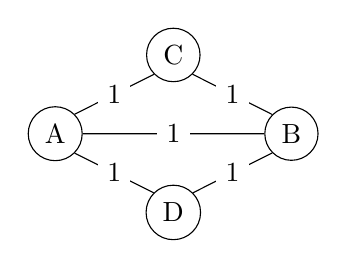
\begin{tikzpicture}[yscale=.5, xscale=.75]
	\node[draw=black, circle] (A) at (0, 0) {A};
	\node[draw=black, circle] (B) at (4, 0) {B};
	\node[draw=black, circle] (C) at (2, 2) {C};
	\node[draw=black, circle] (D) at (2, -2) {D};
	\draw
	(A.north east) -- node[fill=white, rectangle, midway] {$1$} (C.south west)
	(A.south east) -- node[fill=white, rectangle, midway] {$1$} (D.north west)
	(A.east) -- node[fill=white, rectangle, midway] {$1$} (B.west)
	(C.south east) -- node[fill=white, rectangle, midway] {$1$} (B.north west)
	(D.north east) -- node[fill=white, rectangle, midway] {$1$} (B.south west)
	;
\end{tikzpicture}

	\end{minipage}
	\hfill
\end{center}


\smallskip

Similarly, the biharmonic distance arises from the equivalent definition when considering the bi-Laplacian
$\Delta^{2}$ which has the same exact eigenvectors but with squared eigenvalues.
Those two distances can also be defined using a diffusion process (similarly to the equations in the
previous paragraphs), as the expected value of the first arrival at $y$ of a random walk on the mesh
starting at $x$.
For the diffusion distance, the discrete diffusion process used in the definition only considers the
amount of information that has been diffused from $x$ to $y$ and from $y$ to $x$ at time $t$, and is as such
directly tied to the heat equation.

\smallskip

As said, these methods do not contain the geodesics, but may be used as good approximations of the geodesic
distance, or as regularized versions of the geodesic distance.
Moreover, when considering $k$ much smaller than $\nv$, it is easy to approximate the distance quite well
(see Figure \autoref{fig:spectral-approx} below).

\paragraph{Wavefront Propagation}
The hyperbolic wavefront propagation equation (or d'Alembert equation)
\begin{equation*}
	\frac{\d^{2}}{\d t^{2}}u_{t} = c^{2}\Delta u_{t}, \text{or}, \square u = 0
\end{equation*}
where $\square$ is the d'Alembert operator, models the propagation of a wave in a material,
which will again be our surface here.
It arises for example the response of the surface to some elastic deformation $u$ (say, a stone dropping in
a pond) considering the stress tensor $T = E\nabla u$ with $E$ the homogenous modulus of elasticity (here,
the surface tension of the water) and considering the inertial force
$\rho \frac{\partial^{2}u}{\partial t^{2}}$ caused by the local acceleration (the stone moving the water
down on impact).

However, while retrieving distance information from Equations \eqref{eq:heat} and \eqref{eq:poisson} is
not too difficult and doable by solving a simple linear system, retrieving distance from propagating
wavefronts is more easily done from the non-linear hyperbolic eikonal equation
\begin{equation}
	\begin{cases}
		\abs{\nabla u}^{2} = 1 & \text{on } M,         \\
		u = 0                  & \text{on }\partial M,
	\end{cases}\label{eq:eikonal}
\end{equation}
which directly characterizes the distance to the boundary $\partial M$ (which again in our case will be
the set we're computing the distance to).
The eikonal equation arises as the fundamental equation specifying the light paths in space given the
refractive index function of the media encountered.
In our case, there is a unique medium to be considered, and light sources $\partial M$ that emit the light.

\subsection{Implementation Details}
Our input manifold is given as a triangular mesh, that is a set $\V$ of vertices of $\R^{3}$ and a set
$\F \subseteq \left\llbracket 1, \abs{\V}\right\rrbracket^{3}$ of faces passed by indices.
We are also given a set $\partial M$ of sources or boundaries which will be points we compute the distance
to (or from).

\subsubsection{Linear equations}
In the case of linear equations such as Equations \eqref{eq:heat} and \eqref{eq:poisson}, we only have to
construct and solve a linear system of equations from the manifold and the set of sources:

\begin{itemize}
	\item We compute the gradient for the manifold and a function $u$ using the formula of Equation
	      \autoref{eq:facegrad}, as the dynamic array of the face vectors.
	\item We also compute the Laplacian operator for the manifold as the $\nv \times \nv$ matrix using
	      the cotangent formula of Equation \eqref{eq:Laplacian} by iterating on all faces to iterate
	      on all edges and thus all vertices in the end.
	\item If needed, we discretize in time the equation with a single step of backwards Euler method as done
	      in Equation \eqref{eq:discrheat}.
	\item We solve the induced linear system.
\end{itemize}

For the heat equation, we can also retrieve the actual geodesics passing through vertices by solving
in $\phi$ the Poisson equation $\Delta \phi = \div X$ on the normalized gradient $X$ of the temperature
profile.
This is done by simply computing the divergence operator on the manifold from Equation \autoref{eq:divergence},
and iterating on the faces to fill the divergence matrix of the manifold and solving another linear system.
For the Poisson method, a similar transform called the Spalding-Tucker transform exists to better
approximate the geodesics. It is computed by $u \mapsto \sqrt{\abs{\nabla u}^{2} + 2u} - \abs{\nabla u}$.

\smallskip

For the spectral methods, we compute the Laplacian matrix in the same fashion as above, and compute its
eigenspaces (as eigenvalues and eigenvectors).
We then sort those by increasing eigenvalues, skip the first one and compute the approximate geodesic
distance for a given value of $k$.

\subsubsection{Fast Marching Method}
While the simple linear system solving works directly for the heat equation, solving for the geodesic paths
arising from the eikonal equation \eqref{eq:eikonal} is more difficult, as the equation is non-linear, and
thus straightforward system resolution techniques will not work.

To work around this issue, we implemented the fast marching algorithm, based on \cite{kimmelsethian}.
The method initializes the distance at the sources $\partial M$ to $0$ and iterates using a priority queue
on the neighbours of the already seen points.
The distances are not interated according to paths along edges, but so that the eikonal equation is
verified.
If we know values $\phi_{i}, \phi_{j}$ at two corners, we pick $\phi_{k}$ so that the slope of the triangle
$(i, j, k)$ for $\phi$ (so the norm of the gradient of $\phi$, $\left\lVert\nabla \phi\right\rVert$) is $1$
as presented in \autoref{fig:eikonal}.
\begin{figure}
	\usetikzlibrary{shadings}

\begin{tikzpicture}[x={(1, -.2)},z={(.4, .5)},y={(0, 1)}]
	\coordinate (origin) at (0, 0, 0);
	\draw[canvas is xy plane at z=0, ->] (origin) -- +(0, 2) node[above] {$\phi(x)$};
	\draw[canvas is xz plane at y=0] (origin) rectangle +(4, 4);
	%
	\coordinate[canvas is xz plane at y=0] (xi) at (.5, 0, 2.1);
	\coordinate[canvas is xz plane at y=0] (xj) at (3, 0, .6);
	\coordinate[canvas is xz plane at y=0] (xk) at (3.5, 0, 3.1);
	% Draw the triangle
	\fill[canvas is xz plane at y=0, thick, teal!50!purple!20!white] (xi) -- (xj) -- (xk) -- cycle;

	% Draw circles at vertices
	\fill (xi) circle (0.10) node[below left] {$x_i$};
	\fill (xj) circle (0.10) node[below right] {$x_j$};
	\fill (xk) circle (0.10) node[right] {$x_k$};
	%
	\coordinate[canvas is xz plane at y=0] (fxi) at ($(xi) + (0, .9, 0)$);
	\coordinate[canvas is xz plane at y=0] (fxj) at ($(xj) + (0, .7, 0)$);
	\coordinate[canvas is xz plane at y=0] (fxk) at ($(xk) + (0, 1.7, 0)$);
	\fill (fxi) circle (0.10) node[left] {$\phi_i$};
	\fill (fxj) circle (0.10) node[right] {$\phi_j$};
	\fill (fxk) circle (0.10) node[above] {$\phi_k$};

	\draw[dashed] (xi) -- (fxi) (xj) -- (fxj) (xk) -- (fxk);

	\fill[top color=teal, bottom color=purple, opacity=.2] (fxj) -- (fxk) -- (fxi);

	\fill ($(fxi)!1/3!(fxj)!1/3!(fxk)$) circle (0.1) node (bar) {};
	\draw[->, thick] (bar) -- +(-0.133, 0.929, -0.345) node[left] {$\abs{\nabla\phi} = 1$};

\end{tikzpicture}

	\caption{Representation of the Eikonal equation \eqref{eq:eikonal} $\abs{\nabla \phi} = 1$ on a triangular face $(x_i, x_j, x_k)$ of a mesh.}
	\label{fig:eikonal}
\end{figure}
A fun complement to the fast marching algorithm is that when the manifold is flat, i.e. when it is locally
isometric to the Euclidean space, we return to the usual Dijkstra's algorithm.



\subsubsection{Limitations}
\paragraph{Linear PDEs}
The main issue that arises with the linear PDEs we consider is numerical stability.
Indeed, the Laplacian of a manifold will usually be singular, so we need to add regularization terms at
every linear system resolution.
This yields a lot of numerical artifacts when the discretization steps are too big for the precision we
can compute.
Moreover, while the method is polynomial, it scales quite poorly as the number of vertices increases, the
algorithm being in $\mathcal{O}(\nv^{3})$.

\paragraph{Spectral and Poisson Methods}
Some of the issues that arise with those methods are similar to those described above, as they are all based on the linear system solving, a slow process.
However, the main issue with those methods is that they only allow to describe some distance transform from sources or some distance transform on the step.
Those methods are thus not as well adapted to the problem of computing geodesics, although they solve a similar class of problems.

\paragraph{Fast Marching}
For the fast marching algorithm, the method is much shorter, as it runs in (theoretical but impractical)
$\mathcal{O}(\nv \log \nv)$, but this comes at the cost of stability when considering angles that are
too small.
Indeed, the order in which vertices are updated might violate the causality property of the propagation.
If triangles have obtuse angles, there might exist a point $i$ that is closer to the source than another
point $j$, but the distance in $j$ might be finalized before the distance at $i$.
A solution to this exists but might not terminate due to its non-locality as suggested by
\cite{kimmelsethian}, so in general one has to remesh the manifold or apply an iterative strategy as
suggested by \cite{bornemann2000finiteelement}.
Moreover, this algorithm cannot be parallelized, unlike the above methods.

\section{Computational Geometry methods}
\label{sec:comp-geom-methods}
While PDE-based methods provide a general framework to compute geodesic distances on arbitrary, possibly non-meshed manifolds, we can leverage the fact that our manifold is meshed to design more efficient algorithms.
A whole class of such algorithms, arising from computational geometry, can be classified according to two main caracteristics.

\paragraph{Global vs.~local} Global methods compute globally optimal paths, up to numerical precision. Local methods start from an initial non-geodesic path and iteratively improve it until convergence to a local minimum.
\paragraph{Exact vs.~approximate} Exact methods compute the exact geodesic distance, while some approximate methods trade accuracy for speed, and compute only an approximation of the geodesic distance within some guaranteed error bound.
\vspace{5pt}

In the following, we focus on a global and exact method, the Improved Chen-Han algorithm \cite{chen1990shortest,xin2009improving}.

\subsection{Continuous Dijkstra}
The Improved Chen-Han (ICH) algorithm is based on the continuous Dijkstra paradigm introduced by Mitchell et al. for the Mitchell-Mount-Papadimitriou (MMP) algorithm \cite{mitchell1987discrete}.
The main idea is to apply Dijkstra's algorithm in the continuous setting of a piecewise-linear manifold.

A first natural approach could be to consider the graph formed by the vertices and edges of the mesh, and run Dijkstra's algorithm on it. However, this would only yield paths that follow the edges of the mesh, which can be arbitrarily longer than the true geodesic paths on the surface (see \autoref{fig:suboptimal-dijkstra}).

\begin{figure}[ht]
	\centering
	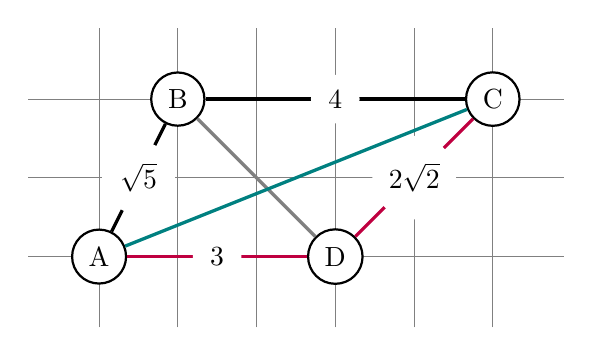
\begin{tikzpicture}
		\draw[step=1.0,gray,thin] (-0.9,-0.9) grid (5.9,2.9);

\begin{scope}[every node/.style={circle,thick,draw,fill=white}]
    \node (A) at (0,0) {A};
    \node (B) at (1, 2) {B};
    \node (C) at (5, 2) {C};
    \node (D) at (3, 0) {D};
\end{scope}

\begin{scope}[>=,every node/.style={fill=white,circle},every edge/.style={draw=black,very thick}]
    \path [->] (A) edge node {$\sqrt{5}$} (B);
    \path [->] (B) edge node {$4$} (C);
    \path [->] (B) edge[draw=gray] (D);
    \path [->] (A) edge[draw=purple] node {$3$} (D);
    \path [->] (D) edge[draw=purple] node {$2\sqrt{2}$} (C);
    
    \path [->] (A) edge[draw=teal] (C);
\end{scope}
	\end{tikzpicture}
	\caption{Example of suboptimality of applying Dijkstra's algorithm on the graph formed by the vertices and edges of the mesh. The \textcolor{purple}{red} path follows the edges of the mesh, while the \textcolor{teal}{green} path is the true geodesic path on the 2D surface, which is shorter.}
	\Description{}
	\label{fig:suboptimal-dijkstra}
\end{figure}

Instead, we would like to consider each point on the surface as a potential node in the graph.
However, since the shortest path on a single face is always a straight line, it is sufficient to only consider points on the edges of the mesh as potential nodes.
This still yields an infinite number of potential nodes; a key concept of the MMP algorithm is to use instead a data structure called \textit{windows}, which encapsulate a continuous interval of points on an edge, along with the information needed to propagate the shortest path from these points to adjacent faces.

Formally, a window
\begin{equation*}
	w = (s, p, e, b_0, b_1, d_0, d_1, \sigma)
\end{equation*}
is defined on edge $e$, between points $b_0$ and $b_1$ (see \autoref{fig:ich-windows}). The window represents shortest paths originating from a ``pseudosource'' $p$, at a distance $\sigma$ from the actual source $s$. Distances from $p$ to the endpoints $b_0$ and $b_1$ of the window, respectively $d_0$ and $d_1$, are also stored.

\begin{figure}
	\centering
	% \includegraphics[width=\linewidth]{images/window-illustration.png}
	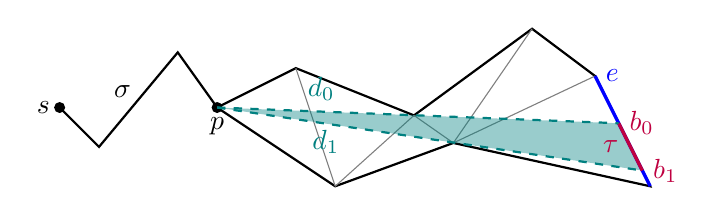
\begin{tikzpicture}
		\coordinate (S) at (1,2);
\coordinate (P) at (3,2);
\coordinate (A) at (4,2.5);
\coordinate (B) at (5.5,1.9);
\coordinate (C) at (7,3);
\coordinate (D) at (7.8,2.4);
\coordinate (E) at (8.5,1);
\coordinate (F) at (6,1.55);
\coordinate (G) at (4.5,1);

\coordinate (A0) at (8.1,1.8);
\coordinate (A1) at (8.4,1.2);

% path from source to pseudo-source
\draw[black, thick] (S) -- (1.5, 1.5) -- (2.5, 2.7) -- (P);
\fill (S) circle (0.07) node[left] {$s$};
\fill (P) circle (0.07) node[below] {$p$};
\node at (1.8, 2.2) {$\sigma$};

\draw[black, thick] (P) -- (A) -- (B) -- (C) -- (D) -- (E) -- (F) -- (G) -- (P);
\begin{scope}[gray]
    \draw (A) -- (G);
    \draw (B) -- (G);
    \draw (B) -- (F);
    \draw (C) -- (F);
    \draw (D) -- (F);
\end{scope}

\fill[teal, opacity=0.4] (P) -- (A0) -- (A1) -- cycle;
\draw[blue, very thick] (D) node[right] {$e$} -- (E);
\draw[purple, very thick] (A0) node[right] {$b_0$} -- (A1) node[right] {$b_1$};

\draw[dashed, teal, thick] (P) -- (A0) node[pos=.2, above right] {$d_0$};
\draw[dashed, teal, thick] (P) -- (A1) node[pos=.2, below right] {$d_1$};
\node[purple] at (8, 1.5) {$\tau$};
	\end{tikzpicture}
	\caption{Illustration of a window $w=(s, p, {\color{blue}e}, {\color{purple}b_0}, {\color{purple}b_1}, {\color{teal}d_0}, {\color{teal}d_1}, \sigma)$.}
	\Description{}
	\label{fig:ich-windows}
\end{figure}

\subsection{Window management and pruning}
While all revolving around the same core idea of continuous Dijkstra, different algorithms differ in how they manage and propagate windows \cite{craneSurvey}.
All \emph{propagate} windows, that is, given a window on an edge, either (a) the window goes through a vertex $v$, and two new windows are created on the two edges adjacent to $v$ in the face opposite to $e$; or (b) the window is contained in the opposite edge, and a single window is kept. However, the different algorithms differ in how they prune and prioritize windows to achieve better theoretical and practical complexity.

The original MMP algorithm does not perform aggressive pruning of windows, but trim overlapping windows on the same edge to avoid redundancy later on; this simple trimming strategy is illustrated in \autoref{fig:window-trimming-mmp}.
It uses a priority queue to always propagate the window with the smallest minimum distance first, ensuring both global optimality and early trimming of redundant windows.
\begin{figure}[ht]
	\centering
	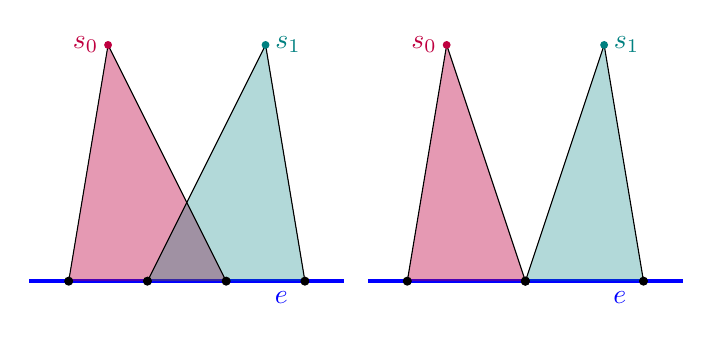
\begin{tikzpicture}
		\coordinate (E00) at (0,0);
\coordinate (E10) at (4,0);

\coordinate (E01) at (4.3,0);
\coordinate (E11) at (8.3,0);

\coordinate (S00) at (1,3);
\coordinate (S10) at (3,3);
\coordinate (S01) at (1+4.3,3);
\coordinate (S11) at (3+4.3,3);

\draw[blue, very thick] (E00) -- (E10) node[pos=0.8, below] {$e$};
\draw[blue, very thick] (E01) -- (E11) node[pos=0.8, below] {$e$};

\fill[purple, opacity=0.4] (S00) -- (0.5,0) -- (2.5,0) -- cycle;
\fill[teal, opacity=0.3] (S10) -- (1.5,0) -- (3.5,0) -- cycle;
\draw[fill] (S00) -- (0.5,0) circle (0.05);
\draw[fill] (S00) -- (2.5,0) circle (0.05);
\draw[fill] (S10) -- (1.5,0) circle (0.05);
\draw[fill] (S10) -- (3.5,0) circle (0.05);
\fill[color=purple] (S00) circle (0.05) node[left] {$s_0$};
\fill[color=teal] (S10) circle (0.05) node[right] {$s_1$};

\fill[purple, opacity=0.4] (S01) -- (0.5+4.3,0) -- (2.0+4.3,0) -- cycle;
\fill[teal, opacity=0.3] (S11) -- (2.0+4.3,0) -- (3.5+4.3,0) -- cycle;
\draw[fill] (S01) -- (0.5+4.3,0) circle (0.05);
\draw[fill] (S01) -- (2.0+4.3,0) circle (0.05);
\draw[fill] (S11) -- (2.0+4.3,0) circle (0.05);
\draw[fill] (S11) -- (3.5+4.3,0) circle (0.05);
\fill[color=purple] (S01) circle (0.05) node[left] {$s_0$};
\fill[color=teal] (S11) circle (0.05) node[right] {$s_1$};
	\end{tikzpicture}
	\caption{Window trimming in the MMP algorithm: overlapping windows on the same edge ${\color{blue}e}$ (left) are trimmed to avoid redundancy (right).}
	\Description{}
	\label{fig:window-trimming-mmp}
\end{figure}

To achieve a better theoretical complexity, the Chen-Han algorithm substitutes the priority queue with a First-In-First-Out (FIFO) queue, propagating windows in the order they were created. To speed up the algorithm in practice, a pruning rule called ``one angle, one split'' is introduced, which we illustrated in \autoref{fig:one-angle-one-split}; however, overlapping windows are not trimmed.

The Improved Chen-Han algorithm combines both approaches, using a priority queue to always propagate the window with the smallest minimum distance first, while also employing the ``one angle, one split'' pruning rule from Chen-Han. Another filtering strategy, illustrated in \autoref{fig:window-trimming}, is introduced to discard windows that cannot lead to shorter paths than already explored window going through the same vertices.

\begin{figure}[ht]
	\centering
	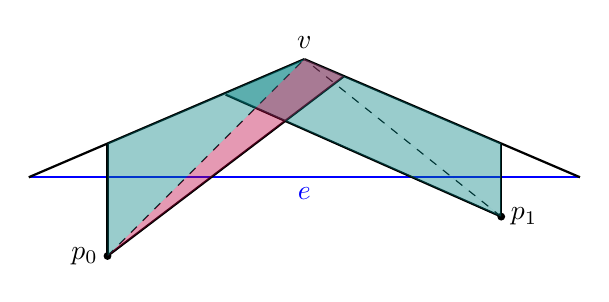
\begin{tikzpicture}
		\coordinate (P0) at (1, -1);
\coordinate (P1) at (6, -0.5);
\coordinate (v) at (3.5, 1.5);
\coordinate (a0) at (1, .43);
\coordinate (a1) at (4, 1.28);
\coordinate (b0) at (2.5, 1.05);
\coordinate (b1) at (6, .43);

\draw[blue, thick] (0, 0) -- (7, 0) node[midway, below] {$e$};
\draw[thick] (0,0) -- (v) node[above] {$v$};
\draw[thick] (7,0) -- (v);

\fill (P0) circle (0.05) node[left] {$p_0$};
\fill (P1) circle (0.05) node[right] {$p_1$};

\draw[thick] (P0) -- (a0);
\draw[thick] (P0) -- (a1);
\draw[thick] (P1) -- (b0);
\draw[thick] (P1) -- (b1);

\draw[dashed] (P0) -- (v);
\draw[dashed] (P1) -- (v);

\fill[teal, opacity=0.4] (P0) -- (a0) -- (v) -- cycle;
\fill[teal, opacity=0.4] (P1) -- (b0) -- (v) -- cycle;
\fill[teal, opacity=0.4] (P1) -- (v) -- (b1) -- cycle;
\fill[purple, opacity=0.4] (P0) -- (v) -- (a1) -- cycle;
	\end{tikzpicture}
	\caption{Illustration of the ``one angle, one split'' pruning rule: if two windows on the same edge ${\color{blue}e}$ split on the same edge $v$, only three out of the four resulting windows are kept, as the one in \textcolor{purple}{red} cannot lead to a shorter path.}
	\Description{}
	\label{fig:one-angle-one-split}
\end{figure}

\begin{figure}[ht]
	\centering
	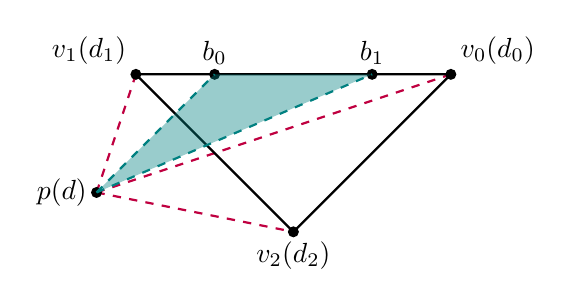
\begin{tikzpicture}
		\coordinate (v0) at (4, 2);
\coordinate (v1) at (0, 2);
\coordinate (v2) at (2, 0);
\coordinate (A) at (3, 2);
\coordinate (B) at (1, 2);
\coordinate (p) at (-0.5, 0.5);

\draw[dashed, thick, purple] (p) -- (v0);
\draw[dashed, thick, purple] (p) -- (v1);
\draw[dashed, thick, purple] (p) -- (v2);

\fill (v0) circle (0.07) node[above right] {$v_0(d_0)$};
\fill (v1) circle (0.07) node[above left] {$v_1(d_1)$};
\fill (v2) circle (0.07) node[below] {$v_2(d_2)$};
\draw[thick] (v0) -- (v1) -- (v2) -- cycle;

\fill (A) circle (0.07) node[above] {$b_1$};
\fill (B) circle (0.07) node[above] {$b_0$};

\fill (p) circle (0.07) node[left] {$p(d)$};
\fill[teal, opacity=0.4] (p) -- (A) -- (B) -- cycle;
\draw[dashed, thick, teal] (p) -- (A);
\draw[dashed, thick, teal] (p) -- (B);
	\end{tikzpicture}
	\caption{Illustration of the window filtering in ICH. For each vertex $v_i$, we denote by $d_i$ the shortest distance to $v_i$ found so far. If one the following inequalities holds, the window $w$ can be safely discarded: $d+\norm{pb_0} > d_0 + \norm{v_0b_1}$, $d+ \norm{pb_1} > d_1 + \norm{v_1b_1}$, or $d+\norm{pb_0} > d_2 + \norm{v_2b_0}$.}
	\Description{}
	\label{fig:window-trimming}
\end{figure}

\subsection{Algorithm outline and example}
We now give a high-level outline of the Improved Chen-Han algorithm, and illustrate it on a toy example.

\textcolor{red}{TODO}


\subsection{Implementation details}
We implemented the Improved Chen-Hand algorithm from scratch in Rust, following the description from \cite{xin2009improving}.
We provide here a short description of some implementation details, data structures used, as well as some difficulties we encountered and limitations of our implementation.

\subsubsection{Data structures}
As other methods, the input of the algorithm is a $2$-manifold represented as a triangle mesh, that is a set of vertices $\V$ and a set of faces ($3$-tuples) $\F$.
However, we also need to represent edges $\E$ explicitly, as windows are defined on edges. We therefore employ an edge data structure, storing for each edge both geometric information (length) and topological information (adjacent faces, vertices, \dots).
Notably, we precompute the twin edges for each edge, which is repeatedly invoked during window propagation.

The main algorithm relies on a priority queue of windows, ordered by the minimum distance from the source to any point in the window.
We implement this priority queue as a binary heap, using Rust's standard library implementation.
Windows are represented as structs containing all the necessary information for propagation, as described above.
Information about the vertices, such as the edge from which the shortest path to the vertex originates, is also stored during the main loop of the algorithm to enable path reconstruction later on.

\subsubsection{Limitations}
Two main limitations of our implementation are worth mentioning: paths along the edges fail to be computed successfully, and some vertices may not receive a distance value at the end of the algorithm when the geometry is particularly complex.

\textcolor{red}{TODO: give an example of challenging geometry on which ICH fails to propagate to all vertices.}

\section{Experiments and results}
\label{sec:experiments}
In this section, we present experiments and results obtained from our implementations of the heat method,
the spectral embedding distance transforms, the fast marching algorithm,
and the Improved Chen-Han algorithm.
All methods being implemented from scratch in the same programming language (Rust),
and optimized up to a similar level, we believe the comparison to be fairly representative of the
practical performances of each algorithm.

The code for all implementations, as well as the scripts to reproduce the experiments, is available at:
\begin{center}
	\href{https://github.com/agroudiev/Geodesic-Paths}{\texttt{https://github.com/agroudiev/Geodesic-Paths}}
\end{center}

\subsection{Methodology}
We collected a set of 27 meshes of various sizes, ranging from 4 to 125'066 vertices.
Mesh come from various sources, including the Thingi10k dataset \cite{zhou2016thingi10kdataset100003dprinting}, filtered to only contain manifolds with a single connected component.
Each mesh was processed by our implementation of each method, starting from a single source vertex chosen arbitrarily.
For each mesh, each algorithm is run 10 times with different source vertices, each point corresponding to the average runtime over these runs.
All experiments were conducted on a MacBook Pro with a 3.22 GHz Apple M1 Pro chip and 32GB of RAM.
Plots are presented on a log-log scale, and when appropriate, a linear regression is fitted to the data points to estimate the practical time complexity of each method.

Care should be taken when interpreting the following results, as the runtime depends on the specific geometry of the meshes used in the benchmark, and may not generalize to all possible meshes.
The number of vertices is not always a fair indicator of the complexity of the geometry, and other factors such as the distribution of vertex valences and curvature may also impact the practical runtime of the algorithm.

\subsection{Benchmarking of linear PDE methods}
\paragraph{Runtime of the Heat Method}
In \autoref{fig:heat-experiments-results}, we present the results of our benchmark of the practical
runtime of the heat method on various meshes.
In theory, the method computes the laplacian in $\O(\nv^{2})$ then solves two linear systems in $\O(n^{3})$.However, we do not observe a clear linear trend in log-log scale as a function of the number of vertices
on the selected range of sizes.
We believe this is due to the overhead of face-gradient, divergence and laplacian operators computation for
small meshes, which takes a lot of added operations, and that the asymptotic behavior would be more
visible on larger meshes.

\begin{figure}[ht]
	\centering
	\includegraphics[width=\linewidth]{images/heat_benchmark.pdf}
	\caption{Benchmark of the time complexity of the \emph{Heat method} on various 3D meshes, as a function of the number of vertices.}
	\Description{}
	\label{fig:heat-experiments-results}
\end{figure}

\paragraph{Precision of Spectral Method}
In \autoref{fig:spectral-approx} we present how well the approximation using $k$ eigenvectors for the
spectral embedding described in \autoref{par:spectral} and the different distance computations
presented in Equation \eqref{eq:spectral} compares to the full precision using the full $n - 1$
eigenvectors non associated to $0$ as an eigenvalue.

The different colours represent the different methods and the different branches for each method are
created from different models.
\begin{figure}[ht]
	\includegraphics[width=\linewidth]{images/accuracy_spectral_methods.pdf}
	\caption{$\ell^{2}$ error of the spectral embedding on $k$ vectors to the full spectral embedding.
		Average computed on most of our manifold examples, as a function of the percentage of the dimension
		$\nv$ used for the embedding size.}
	\label{fig:spectral-approx}
\end{figure}

In terms of runtime, the duration is similar to the heat method as most of the computation time is spent
computing the laplacian of the manifold, as well as its eigenspace decomposition which is, in theory,
equivalent in time to the computation of a matrix multiplication (and thus near the resolution of a linear
system).

\subsection{Runtime of Fast Marching}
The fast marching algorithm works really similarly to Dijkstra's algorithm by computing locally shortest
paths.
As such, it only approximates geodesics (from the approximation on the mesh), but does so by performing at
most one $\O(1)$ operation on the minimum element of a priority queue on the vertices, which can be one
vertex at most once.
As such, in theory the algorithm runs in $\O(\nv\log\nv)$ when using a fully optimal priority queue.
\autoref{fig:fastmarching-experiments-results} shows that the default implementation in Rust of the
priority queues is actually a bit slower\footnote{This is because the \texttt{BinaryHeap} data structure
	can be dynamically allowed and is as such a bit slower than the theoretical optimum speed.}
and the algorithm thus runs in $\O(\nv\sqrt{\nv})$ which is still sub-quadratic.

\begin{figure}[ht]
	\centering
	\includegraphics[width=\linewidth]{images/fastmarching_benchmark.pdf}
	\caption{Benchmark of the time complexity of the \emph{Fast Marching algorithm} on various 3D meshes, as a function of the number of vertices. Slope: $1.51$, $r^2$: $0.98$.}
	\Description{}
	\label{fig:fastmarching-experiments-results}
\end{figure}

\subsection{Runtime of the ICH algorithm}
Theoretically, the Improved Chen-Han algorithm runs in $\mathcal{O}(n^2 \log n)$ time on a mesh with $n$ vertices, which is worse than the $\mathcal{O}(n^2)$ previously obtained by the Chen-Han algorithm, the $\log n$ factor coming from the priority queue management.
\todo{Overfull hbox}

\cite{craneSurvey} reports that in practice, the ICH algorithm runs in sub-quadratic time on average, and dramatically improves the performance of the original Chen-Han algorithm, without supporting such a claim with a precise benchmark. We therefore conducted experiments to benchmark the practical runtime of our implementation of the ICH algorithm on various meshes, and report the results in \autoref{fig:ich-experiments-results}.

\begin{figure}[ht]
	\centering
	\includegraphics[width=\linewidth]{images/ich_benchmark.pdf}
	\caption{Benchmark of the time complexity of the \emph{ICH algorithm} on various 3D meshes, as a function of the number of vertices. Slope: $1.60$, $r^2$: $0.96$.}
	\Description{}
	\label{fig:ich-experiments-results}
\end{figure}

The results confirm the sub-quadratic practical runtime of the ICH algorithm, with a fitted slope of $1.60$ on a log-log scale, corresponding to a time complexity of approximately $\mathcal{O}(n^{1.60})$ in practice.

\subsection{Comparison and discussion}
In \autoref{tab:summary} we present a short summary of all the methods we discussed in this report,
as well as their limitations and time complexities.

\newcommand\intertitre[1]{%
	\SetRow{rowsep=1pt,bg=teal!10}
	\SetCell[c=5]{mode=text,l,font=\itshape\footnotesize}
	#1 &
}
\begin{table}[ht]
	\begin{tblr}[expand=\intertitre]{%
		rowspec={Q[m]Q[m]Q[m]Q[m]Q[m]Q[m]Q[m]Q[m]},
		colspec={Q[co=1,c]Q[co=1.5,mode=math,c]Q[mode=math,co=1.5,c]Q[co=1,c]Q[c, co=1.5, cmd=\scriptsize]},
		row{3, 5, 8}={bg=teal!20!white},
				row{1}={c,cmd=\textbf,mode=text,fg=white,bg=teal},
				colsep=3pt,
				hline{-},
				vline{1, 2, 6},
			}%
		Method        & Theoretical Runtime & Actual Runtime    & Precision & \small Limitations                                              \\
		\intertitre{PDE-based methods}                                                                                                        \\
		Heat          & \O(\nv^{3})         &                   & Approx.   & Stability, runtime, fixed sources, no paths                     \\
		Poisson       & \O(\nv^{3})         &                   & Approx.   & Stability, not true geodesics, runtime, fixed sources, no paths \\
		Spectral      & \O(\nv^{3})         &                   & Approx.   & Stability, not true geodesics, runtime, no paths                \\
		Fast Marching & \O(\nv\log \nv)     & \O(\nv\sqrt{\nv}) & Approx.   & Fixed sources, limited meshes, no paths                         \\
		\intertitre{Computational geometry methods}                                                                                           \\
		ICH           & \O(\nv^{2}\log \nv) & \O(\nv^{1.6})     & Exact     & Limited meshes \textcolor{red}{\@ antoine vérifie stp}
	\end{tblr}
	\caption{Summary table comparing the different methods, their limitations and time complexity}
	\label{tab:summary}
\end{table}

We see in the table that two methods stand out: the Fast-Marching algorithm and the
Improved Chen-Han algorithm which both run in around $\O(\nv^{1.5})$ time in practice.
However, while the fast marching algorithm only allows to compute the distance from a fixed set of sources,
the Improved Chen-Han algorithm computes all distances with better precision at the cost of a higher
theoretical runtime, which in practice does not matter when pruning is done properly.

\section*{Conclusion}
In this report, we investigated different methods to compute shortest-paths on meshed $2$-manifolds embedded in $\R^{3}$.
We presented two classes of methods: PDE-based methods, which solve physical equations on the manifold to retrieve geodesic distances, and computational geometry methods, which leverage the meshed structure of the manifold to design efficient algorithms.
We provided from-scratch implementations of three methods: the heat method, fast marching, and the Improved Chen-Han algorithm, and compared their practical performances on various datasets of meshes.
Our experiments brought to light the practical runtime of each method, as well as their respective strengths and limitations.

\appendix
\bibliography{report}
\end{document}
